\section{Method}\label{sec:method}
% Implementation facts below were read from the code on 2026-10-29: semseg/models/reliadino/{encoder,fusion,model,hires_adapter}.py,
% train_reliadino.py (two-pass loop l.1000-1110, _qaf_kd_kl l.283), semseg/datasets/degrade.py (TRAIN_OPS l.159),
% config configs/lecun-deliver_rgbdel_P46_c3only_seed20260821_screen40_A2hires.yaml.

Fig.~\ref{fig:arch} summarizes \ours{}. The model keeps a single foundation backbone frozen and shares it across all sensors, so that every sensor is read with the same visual vocabulary. It adds a small number of trained components around the backbone: sensor-specific low-rank adapters, a symmetric cross-modal fusion, a decoder with a high-resolution path, and two complementary heads. Training uses every batch twice, once clean and once with synthetic sensor degradation, and distills a frozen clean-trained teacher into the degraded pass.

\begin{figure*}[t]
\centering
% Source: figures/src/fig_arch_standalone.tex + latex/figures/fig_arch.tex (TikZ), built by build.sh.
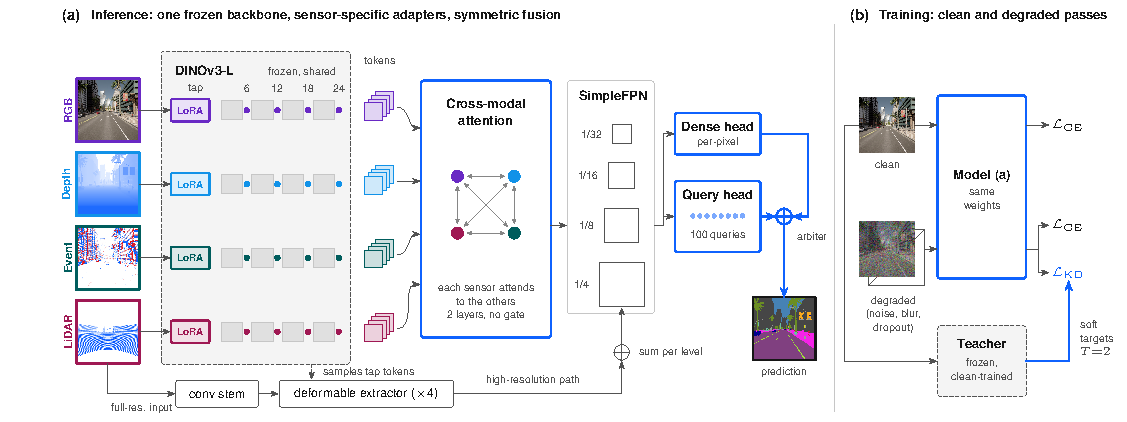
\includegraphics[width=\textwidth]{figures/fig_arch.pdf}
\caption{Overview of \ours{}. (a) Each sensor passes through the same frozen DINOv3-L with its own LoRA adapter; tokens from four depths are fused by symmetric cross-modal attention, decoded by a SimpleFPN augmented with a high-resolution path, and classified by a dense head and a query head combined by an arbiter. (b) Every batch is used twice: a clean pass and a synthetically degraded pass, the latter also distilled from a frozen teacher trained on clean data. Blue outlines mark trained components; dashed boxes are frozen. The scene and the prediction are a DELIVER test image and the output of our model. \todo{draft drawn by the paper session; redraw per notes/figure\_guide.md}}
\label{fig:arch}
\end{figure*}

\subsection{Frozen Backbone with Sensor-Specific Adapters}
Let $x_s$ denote the input of sensor $s\in\{1,\dots,S\}$, converted to a three-channel image (Section~\ref{sec:exp}). Every $x_s$ is processed by the same DINOv3 ViT-L/16 backbone~\cite{dinov3_2025}, whose weights are frozen. To let each sensor adapt the shared features to its own statistics, we attach a separate low-rank adapter (LoRA)~\cite{lora2022} of rank 8 to the attention projections of the backbone for each sensor. Instead of reading only the last layer, we take the token maps after blocks 6, 12, 18, and 24, so that the decoder receives both low-level and semantic evidence; each of the four maps is projected by a sensor-specific $1\times1$ layer. The result is a stride-16 token set $T_s$ for every sensor.

\subsection{Symmetric Cross-Modal Fusion}
Many fusion designs nominate RGB as the primary stream and inject the other sensors into it~\cite{cmx2023,mmsamadapter2025}, which makes the model fragile exactly when RGB fails. We instead treat the sensors symmetrically. In each of two fusion layers, the tokens of sensor $s$ form the queries of a multi-head attention whose keys and values are the tokens of all other sensors,
\begin{equation}
T_s \leftarrow T_s + \mathrm{MHA}\big(T_s,\ [T_{s'}]_{s'\neq s},\ [T_{s'}]_{s'\neq s}\big),
\end{equation}
followed by a feed-forward layer. No sensor is privileged, and the attention has no gate and receives no external reliability signal. The fused tokens of all sensors are merged by a gated MLP into one stride-16 feature map $F$. In addition, a per-class sensor router inherited from earlier versions of our model adds a zero-initialized residual term to the logits. \todo{decide with the method session how to describe the router (MODEL.ROUTER = per-class reliability-anchored modality router, fusion.py:64) and whether it needs its own ablation row; earlier internal measurement: about +0.1 mIoU}

\subsection{Decoder with a High-Resolution Path}
A SimpleFPN~\cite{vitadapter2023} turns $F$ into a feature pyramid at strides 4, 8, 16, and 32. Because every level is interpolated from stride-16 tokens, structures thinner than a token, such as poles and pedestrians at a distance, are poorly represented. We therefore add a high-resolution path that follows the adapter used in the official DINOv3 segmentation code~\cite{dinov3_2025,vitadapter2023}. A convolutional stem with weights shared across sensors (and a sensor-specific $1\times1$ projection) extracts multi-scale features from the raw inputs. Four deformable-attention extractors then let these convolutional queries sample semantic evidence from the four tapped token maps. Unlike the original adapter, we use only the extractors and do not inject anything back into the backbone, which stays untouched. The path's output is added to the FPN levels without a gate. We regard this path as an engineering complement taken from prior work, not as a contribution, and we analyze where its gain comes from in Section~\ref{sec:analysis}.

\subsection{Dense and Query Heads}
Two heads read the pyramid. A dense convolutional head classifies every pixel at stride 4. A Mask2Former-style query head~\cite{mask2former2022} with 100 queries and six decoder layers predicts class scores and masks, which are converted into per-pixel class scores $Q$. An arbiter combines the two with a learned per-class weight $\lambda_k$ that is initialized at zero,
\begin{equation}
\ell_k(p) = D_k(p) + \lambda_k\, Q_k(p),
\end{equation}
so that the query head contributes only where it helps the dense prediction.

\subsection{Two-Pass Training with Teacher Distillation}
Our analysis in Section~\ref{sec:analysis} shows that over-reliance on one sensor is learned from clean training data. We therefore change the training signal rather than the architecture. Every batch $(x, y)$ is used twice. The clean pass computes the segmentation loss $\mathcal{L}_{\mathrm{seg}}(f(x), y)$. The degraded pass builds $\tilde{x}$ by corrupting each sensor of each sample independently with probability 0.5; one fifth of the corrupted sensors are removed entirely (zero-filled), and the rest receive one operator drawn from a sensor-specific set: patch dropout, blur, gain and gamma changes, colour shift (RGB), depth holes (depth), beam dropout (LiDAR), and resolution loss (event). The corruption strength follows a curriculum that rises from 0.3 to 0.6 and 1.0 of its maximum at epochs 0, 10, and 20. Gaussian and salt-and-pepper noise are deliberately excluded from training so that the noise evaluation tests generalization to unseen corruption.

The degraded pass is supervised by the labels and by a frozen teacher $g$, a model of the same architecture without the high-resolution path that was trained on clean data only. The teacher sees the clean input, and its soft predictions are distilled into the degraded pass:
\begin{equation}
\begin{split}
\mathcal{L} ={} & \mathcal{L}_{\mathrm{seg}}(f(x), y) + \mathcal{L}_{\mathrm{seg}}(f(\tilde{x}), y)\\
& + \alpha\, T^2\, \mathrm{KL}\!\left(\sigma\!\left(\tfrac{g(x)}{T}\right) \Big\|\, \sigma\!\left(\tfrac{f(\tilde{x})}{T}\right)\right),
\end{split}
\end{equation}
with $\alpha=0.5$ and $T=2$, where $\sigma$ is the softmax over classes and the Kullback--Leibler divergence is averaged over pixels. The scheme needs no condition labels and no degradation labels, and it adds no computation at inference. Its parts are known: clean-teacher distillation and synthetic dropout appear in robust multimodal segmentation~\cite{anyseg2024,rmmss2025}. Our point is not a new loss but the evidence that this change of training signal, and not the architecture, removes the sensor over-reliance (Section~\ref{sec:analysis}).
